\documentclass[a4paper,11pt]{article}%
    
\usepackage{fullpage}%
\usepackage[T1]{fontenc}%
\usepackage[utf8]{inputenc}%


\usepackage[french]{babel}% % Adjust the main language


\usepackage{graphicx}%
\usepackage{url}%
\usepackage{abstract}%
\usepackage{lipsum}
\usepackage{mathpazo}%
\usepackage{multicol}
\usepackage{listings}%
\usepackage[linesnumbered,ruled,vlined]{algorithm2e}
\usepackage{subcaption}

\parskip=0.5\baselineskip



\sloppy

\begin{document}

\title{Rapport de stage}

\author{Clément Legrand-Lixon}

\maketitle


\section*{Introduction}
Le Vehicle Routing Problem (VRP), consiste à relier un nombre $n$ de clients par des tournées, commençant et finissant toutes à un même point défini, le dépôt. 
Ce problème est NP-complet, et dispose de nombreuses applications dans le monde d'aujourd'hui (notamment gestion d'un réseau routier). 
D'autant plus que ce problème dispose de nombreuses variantes (ajout d'une contrainte de temps, plusieurs dépôts possibles...). 
L'une des variantes les plus connues consiste à prendre en compte pour chaque client sa demande, de sorte à ce que les tournées créées ne dépassent pas une certaine capacité définie à l'avance. 
On nomme ce problème Capacitated Vehicle Routing Problem (CVRP). 

Si de nombreuses heuristiques ont vu le jour pour résoudre ce problème, aucune d'entre elles ne parvient à trouver des solutions optimales pour toutes les instances de la littérature, malgré de très bons résultats dans la plupart des cas. Récemment~\cite{Sorensen_2017}, une nouvelle heuristique efficace a vu le jour. L'objectif de mon stage est de créer une \emph{Learning Heuristic} afin de trouver de meilleures solutions.

Ce rapport commence par présenter le problème étudié, et introduit les notations et opérateurs utilisés dans la suite. Il présente ensuite l'objectif du stage et la méthode mise en place pour y parvenir. 
Différents problèmes sont alors soulevés, et sont traités dans chacune des parties qui suit.
  

\section{Présentation des notions et notations}
Cette partie introduit le problème étudié ainsi que les différentes notations utilisées ensuite dans le reste du rapport. 

\subsection{Description du problème}
Le problème étudié ici (CVRP) est une extension du problème (VRP). Ces problèmes font partie de la famille des problèmes d'optimisation stochastique.

\subsubsection{Problèmes d'optimisations}

\subsubsection{Vehicle Routing Problem (VRP)}

Le problème de tournées de véhicules, est un problème NP-complet, où sont donnés $n$ points de coordonnées $(x_i,y_i)$, représentant 1 dépôt et $n-1$ clients. $k$ véhicules sont disponibles. 
L'objectif est alors de minimiser la longueur du réseau (ensemble des tournées). 
On définit alors $x_{i,j}^v$ qui vaut 1 si $j$ est desservi après $i$ par le véhicule $v$, et 0 sinon. 
On définit également $c_{i,j}$ comme étant la distance entre $i$ et $j$.
Il faut donc déterminer la solution $Sol$ vérifiant :
\begin{center}
$ Sol = argmin_{Sol} \sum_{i = 0}^{n} \sum_{j = 0}^{n} \sum_{v = 1}^{k} c_{i,j} x_{i,j}^v = argmin_{Sol}cost(Sol)$
\end{center}

Les tournées créées doivent également respecter les contraintes suivantes :
\begin{itemize}
\item Chaque client doit être desservi par une et une seule tournée;
\item Chaque tournée doit partir et s'arrêter au dépôt.
\end{itemize}

Un exemple d'instance est présenté en figure~\ref{Instance3205}, où les points rouges représentent les clients et le point bleu le dépôt. Une solution possible au problème est représenté en figure~\ref{SNC3205} mais n'est à priori pas optimale. 
De nombreux algorithmes ont vu le jour pour tenter de résoudre ce problème, ainsi que les nombreuses variantes qui existent (ajout de contraintes de capacité, temps ou longueur sur les tournées, ces contraintes sont cumulables). 
C'est l'ajout de capacité aux tournées qui nous intéressera plus particulièrement.


\begin{figure}

\centering
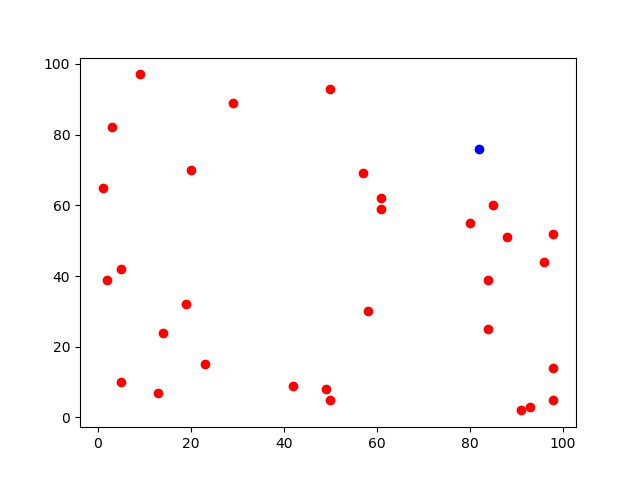
\includegraphics[scale=0.5]{Instance.png}
\caption{Représentation de l'instance A-n32-k05 de la littérature}
\label{Instance3205}
\end{figure}

\begin{figure}

\centering
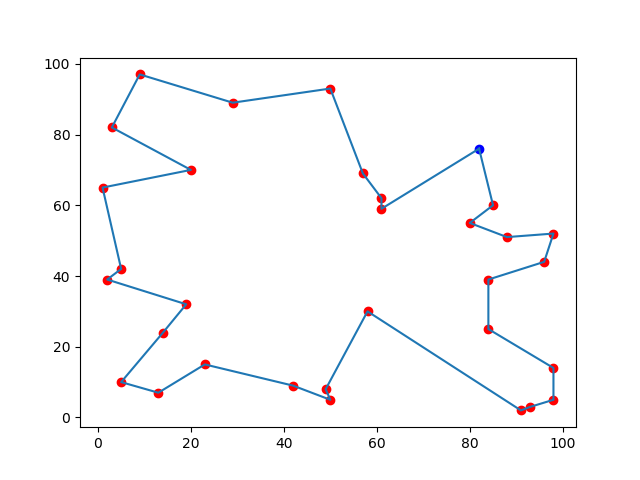
\includegraphics[scale=0.5]{solutionNoCapacity.png}
\caption{Représentation d'une solution de l'instance A-n32-k05}
\label{SNC3205}
\end{figure}

\subsubsection{Capacitated VRP (CVRP)}

On étend le VRP au CVRP en ajoutant à chaque client $i$ une demande $d_i$, ainsi qu'une capacité $C$ aux véhicules.
Une nouvelle contrainte vient donc s'ajouter aux contraintes classiques du VRP :
\begin{itemize}
\item La demande totale sur chaque tournée ne doit pas excéder la capacité du véhicule.
\end{itemize}
Si on reprend l'instance A-n32-k05, en considérant les demandes des clients ainsi que la capacité disponible pour chaque véhicule, on obtient une solution présente sur la figure~\ref{SC3205}, qui n'est pas optimale. 
Ce problème est beaucoup étudié car il a de nombreuses applications (comme par exemple la gestion du trafic routier, ou alors la gestion d'un réseau de bus), et peu de solutions optimales ont été trouvées pour des instances de plus de $500$ clients. 

\begin{figure}
\centering
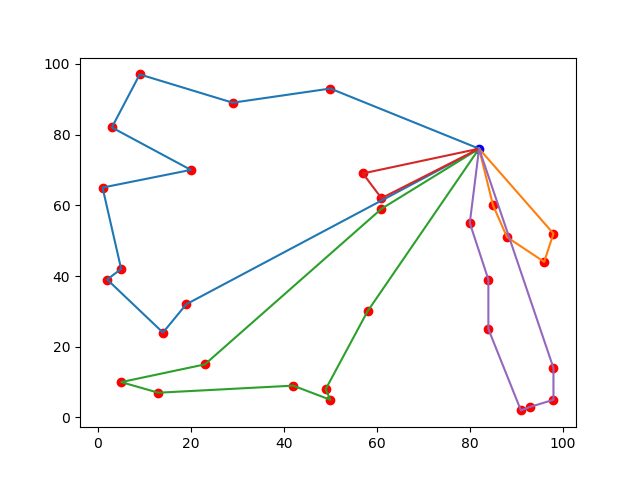
\includegraphics[scale=0.5]{solutionCapacity.png}
\caption{Représentation d'une solution de l'instance A-n32-k05, où les demandes des clients sont prises en compte}
\label{SC3205}
\end{figure}

\subsection{Parcours et exploration des voisinages}
\label{voisinage}

Lorsqu'il s'agit de trouver une solution optimale à un problème, il est souvent intéressant d'explorer les voisinages d'une solution pour voir s'il n'y a pas mieux. Selon la méthode d'exploration employée, il peut être intéressant de parcourir le voisinage de différentes manières, pour ne pas toujours favoriser les mêmes voisins.

L'\underline{exploration} d'un voisinage de solutions peut être plus ou moins exhaustif selon la condition d'arrêt utilisée.
On distingue principalement, deux conditions d'arrêt lorsqu'il s'agit d'explorer des voisinages :

\begin{itemize}
\item First improvement (\emph{FI}) : on parcourt le voisinage jusqu'à trouver un changement qui améliore la solution actuelle (on s'arrête donc à la première amélioration trouvée);
\item Best improvement (\emph{BI}) : on parcourt tout le voisinage, et on applique le changement qui va le plus améliorer notre solution actuelle. \\
\end{itemize}

Pour explorer un voisinage, on peut le \underline{parcourir} de différentes manières de sorte à ne pas toujours favoriser les mêmes voisins. On considérera ici 3 parcours différents : 

\begin{itemize}
\item Dans l'ordre (\emph{O}) : les voisins sont parcourus dans un ordre naturel (du premier au dernier);
\item Dans un semi-ordre (\emph{SO}) : on commence le parcours là où on s'était arrêté au dernier parcours, on parcourt ensuite les voisins dans l'ordre;
\item Aléatoirement (\emph{RD}) : on tire aléatoirement l'ordre dans lequel on va parcourir les voisins. \\
\end{itemize}

On peut remarquer que peu importe le parcours effectué, pour faire une exploration \emph{BI}, il faudra passer par tous les voisins. Pour qu'une exploration \emph{FI} soit efficace, il faut éviter un parcours \emph{O}, car dans ce cas on privilégie une certains voisinages qui seront choisis plus souvent. On retiendra le tableau récapitulatif suivant:

\begin{center}
\begin{tabular}{|c|c|c|}
   \hline
     & \emph{BI} & \emph{FI}  \\
   \hline
   \emph{O} & Oui & Non \\
   \hline
   \emph{SO} & Non & Oui \\
   \hline
   \emph{RD} & Non & Oui  \\
   \hline
\end{tabular}
\end{center}


\subsection{Motivation et objectif}

L'objectif de mon stage d'intégrer de la connaissance à un algorithme d'optimisation utilisé pour résoudre CVRP, afin de le rendre plus performant.
Une idée pour y parvenir serait de réussir à prédire des arêtes qui appartiendront à la solution optimale, en n'observant que des solutions initiales que l'on peut générer rapidement. 
On pourra ensuite exploiter ces arêtes pour construire une nouvelle solution.
Nous adopterons la méthodologie suivante pour atteindre notre objectif :
\begin{itemize}
\item Comparer des solutions initiales à des solutions optimales pour des petites instances;
\item Établir de l'étude précédente des règles qui permettent de caractériser ces arêtes;
\item Exploiter les arêtes obtenues dans un algorithme d'optimisation.
\end{itemize}

Cette méthode, nous impose de résoudre les problèmes suivants : Comment construire une solution initiale de bonne qualité ? Quel algorithme d'optimisation utiliser ? Comment extraire la connaissance ? Comment intégrer la connaissance dans l'algorithme d'optimisation retenu ?

\section{Construction d'une solution initiale de bonne qualité}
Pour construire une solution initiale nous allons utiliser la dernière version d'un algorithme très répandu dans la littérature : l'algorithme Clarke \& Wright~\cite{Altinel_2005}.

\subsection{Description de l'algorithme}
L'algorithme Clarke \& Wright (CW) est un algorithme glouton. 
Initialement chaque client est desservi par un véhicule (de cette manière la contrainte sur le nombre de véhicules disponibles n'est pas respectée). Ensuite les tournées sont fusionnées en fonction des \emph{savings} calculées.
On définit le \emph{saving} des clients $i$ et $j$ de la manière suivante :

\begin{center}
$s(i,j) = c_{i0} + c_{0j} - \lambda c_{ij} + \mu \vert c_{i0} - c_{0j} \vert + \nu \frac{d_i + d_j}{\overline{d}}$
\end{center}

Les paramètres $(\lambda, \mu, \nu)$ jouent un rôle important dans la formule précédente, ce que nous verrons plus tard. (rôle des paramètres à détailler). 

L'algorithme \ref{algo:CW} présente le fonctionnement de l'algorithme CW.

\begin{algorithm}
\DontPrintSemicolon % Some LaTeX compilers require you to use \dontprintsemicolon instead
\KwIn{Un ensemble de points I, un ensemble d'entiers $D = {d_1,...,d_n}$ et un triplet $(\lambda,\mu,\nu)$ de flottants}
\KwOut{Une solution au problème I}

\For{$i \gets 1$ \textbf{to} $n$} {
	$Sol \gets Sol \cup [0,i,0]$\;
}
Calculer les savings de toutes les arêtes\;

\While {max$_{i,j} s(i,j) > 0$} {
	$(i,j) \gets argmax_{(i,j)} s(i,j)$\;
	$r_i \gets findRoute(Sol,i)$\;
	$r_j \gets findRoute(Sol,j)$\;
	\If{$r_i$ et $r_j$ peuvent fusionner} {
		Retirer $r_i$ et $r_j$ de $Sol$\;
		Si possible fusionner $r_i$ et $r_j$\;
		Ajouter le résultat dans $Sol$ et mettre $s(i,j) = 0$\;
	}
}

\Return{$Sol$}\;
\caption{{\sc Clarke-Wright} calcule une solution initiale}
\label{algo:CW}
\end{algorithm}

Exemple d'exécution de l'algorithme avec $(\lambda, \mu, \nu) = (1,1,1)$, sur l'instance A-n37-k06, représenté sur les figures \ref{CWinit} à \ref{resCW101010}.

\begin{figure}
\begin{center}




  	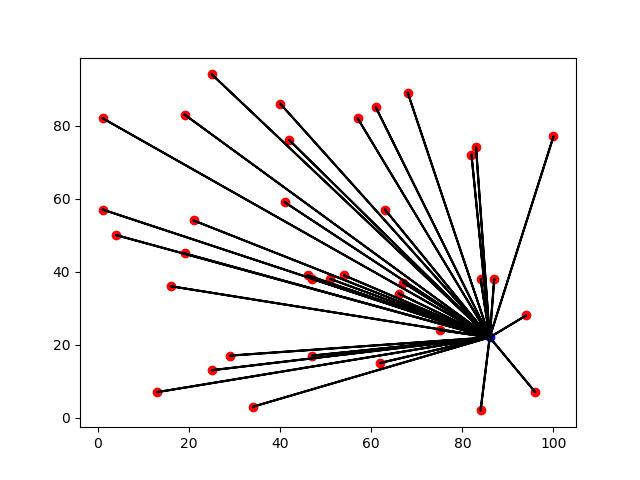
\includegraphics[scale=0.4]{CWinit.png}
  	\caption{Initialisation}
	\label{CWinit}
	
  
  
	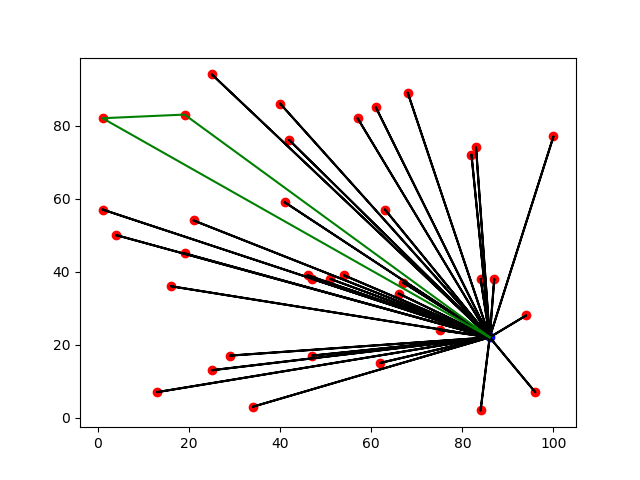
\includegraphics[scale=0.4]{CW1.png}
	\caption{1$^{ere}$ fusion}
 	\label{CW1}
  	


	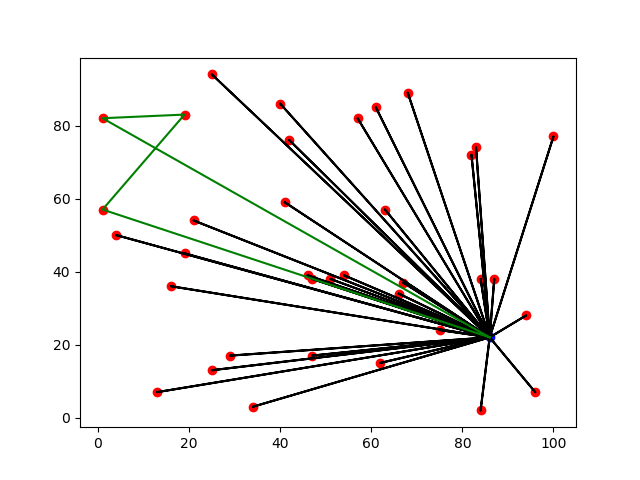
\includegraphics[scale=0.4]{CW2.png}
	\caption{2$^{eme}$ fusion}
	\label{CW2}


	 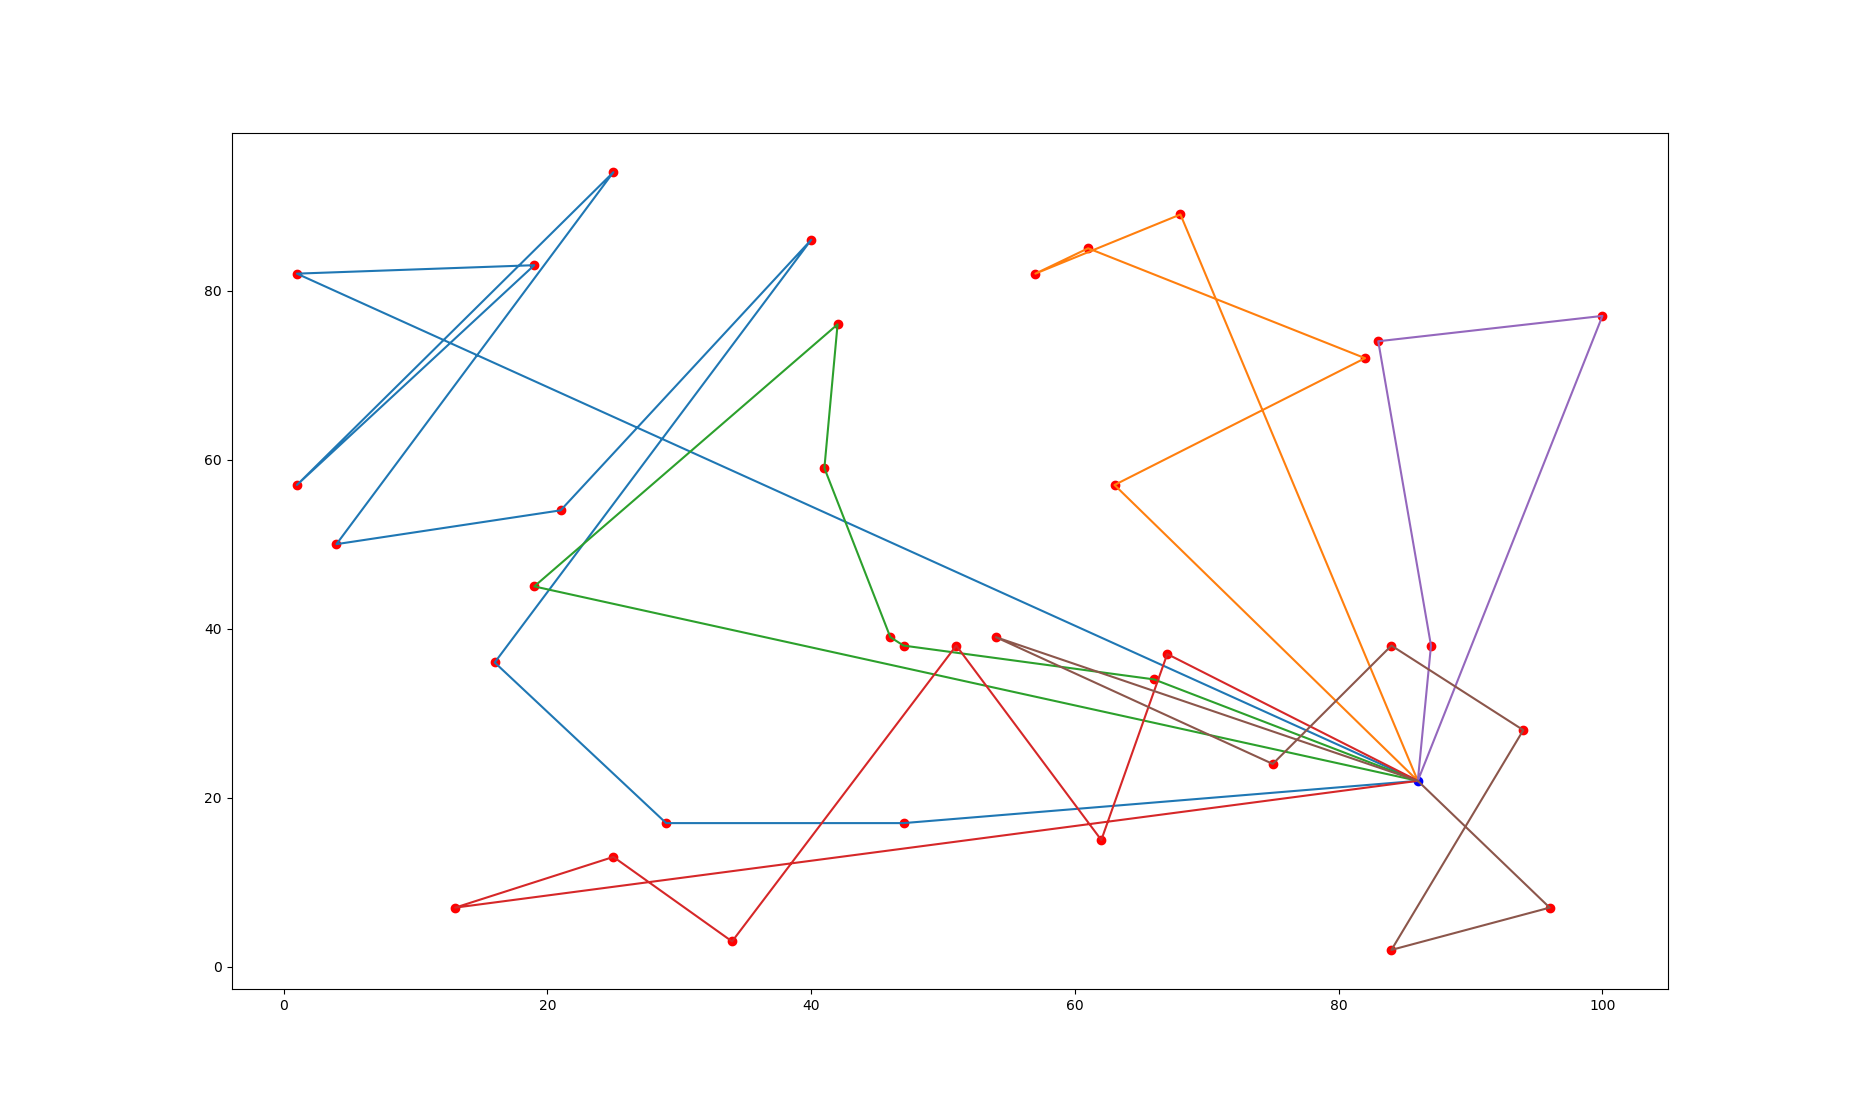
\includegraphics[scale=0.15]{resCW101010.png}
	 \caption{Solution obtenue, $cost = 1297$}
	\label{resCW101010}

\end{center}
\end{figure}


 
\subsection{Choix des paramètres $(\lambda, \mu, \nu)$}
Le triplet $(\lambda, \mu, \nu)$ a déjà été étudié de nombreuses fois dans la littérature. L'article~\cite{Altinel_2005} précise qu'il suffit de considérer $(\lambda, \mu, \nu)$ dans $]0,2] \times [0,2]^2$ pour avoir de bonnes solutions. 
Par ailleurs, il est inutile de considérer  

\section{Proposition d'un algorithme d'optimisation}

\section{Extraction de la connaissance}

\section{Intégration de la connaissance} 

\bibliographystyle{plain}
\bibliography{biblio}
\end{document}